% !TEX root = ../TAMU_Thesis_Main.tex

%%%%%%%%%%%%%%%%%%%%%%%%%%%%%%%%%%%%%%%%%%%%%%%%%%%%%%%%%%%%%%%%%%%%%%
%%                           SECTION IV
%%%%%%%%%%%%%%%%%%%%%%%%%%%%%%%%%%%%%%%%%%%%%%%%%%%%%%%%%%%%%%%%%%%%%

\chapter{SUMMARY AND CONCLUSIONS \label{cha:Summary}}

The summary goes here, along with your conclusions. The title of this final chapter/section must contain the words ``summary'' or ``conclusions.''

Here, I attempt to fill the section with more figures, possibly more tables. The inclusion of these floats is to manipulate the list of figures and list of tables in order to see when the inconsistent spacing begins. It is important to remember that any images you wish to use are placed in the appropriate directory inside the folder in which the project is kept. In the original template, all the images used as figures here are placed in the subdirectory \textit{graphics}, as declared in the preamble of \textit{TAMU\_Thesis\_Main.tex}. If you wish to use any other directories, be sure to declare them in the preamble of \textit{TAMU\_Thesis\_Main.tex}. See the figure below on how to declare directories.

\begin{figure}[ht]
	\centering
	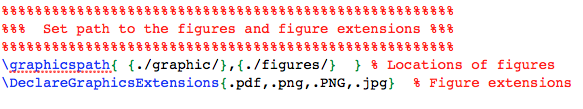
\includegraphics[width=\textwidth]{GraphicDir}
	\caption{Declaring graphics directories and image extensions.}
\end{figure}

The template has a section to place any packages that you are using (\figref{fig:custom_packages}). By default, the hyperref, multirow, footnote, amsthm, and url packages are all loaded in this area. The hyperref package enables hyper references within the document, i.e., if you click on a section in the table of contents, or on a figure, table, equation number, you will be taken to the section's, figure's, table's, equation's location in the document. The multirow package provides commands to place table entries across multiple rows. And so on...

\newpage%force newpage

\begin{figure}[t]
	\centering
	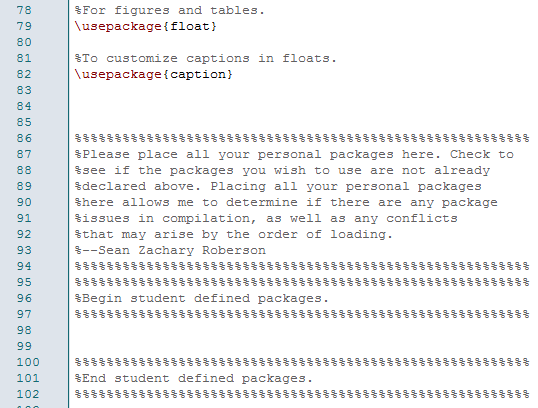
\includegraphics[width=\textwidth]{CustomPackage}
	\caption{The place to declare any packages you require that I have not already declared. This simplifies debugging.}
	\label{fig:custom_packages}
\end{figure}

There is also a section in the \textit{TAMU\_Thesis\_Main.tex} document that allows for custom commands (\figref{fig:custom_commands}). In this case the command {\it mmday} has been defined, which produces \mmday. Defining commands like this can be very useful when a certain string is used very often, or a complex equation format is needed many times. In the case of the units for millimeters per day, we no longer have to write
\begin{verbatim}
mm day$^{-1}$
\end{verbatim}
every time we need the units. We only need to type
\begin{verbatim}
\mmday
\end{verbatim}
Note that if there is a space required between the units and text, add a backslash to the end of the command for the space to appear. For example, there is no space with \mmday even when a space is present after the command. However, if we add a backslash after \mmday\ a space is added.

\begin{figure}[ht]
	\centering
	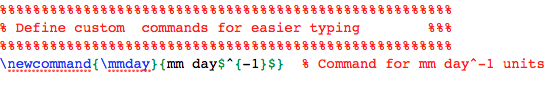
\includegraphics[width=\textwidth]{CustomCommands}
	\caption{The place to declare custom commands.}
	\label{fig:custom_commands}
\end{figure}

\begin{figure}[!b]
	\centering
	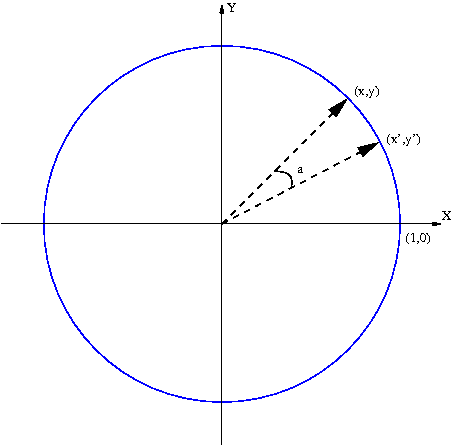
\includegraphics[width=0.8\textwidth]{CartesianCoordinate.png}
	\caption{Two points on the unit circle and their corresponding position vectors. This figure should be at the bottom of the page}
\end{figure}

This section has filler text. These words serve no meaning except to fill a few lines in the document. This section has filler text. These words serve no meaning except to fill a few lines in the document. This section has filler text. These words serve no meaning except to fill a few lines in the document. This section has filler text. These words serve no meaning except to fill a few lines in the document. This section has filler text. These words serve no meaning except to fill a few lines in the document. This section has filler text. These words serve no meaning except to fill a few lines in the document. This section has filler text. These words serve no meaning except to fill a few lines in the document. This section has filler text. These words serve no meaning except to fill a few lines in the document. This section has filler text. These words serve no meaning except to fill a few lines in the document. This section has filler text. These words serve no meaning except to fill a few lines in the document. This section has filler text. These words serve no meaning except to fill a few lines in the document. This section has filler text. These words serve no meaning except to fill a few lines in the document.

\begin{figure}[!b]
	\centering
	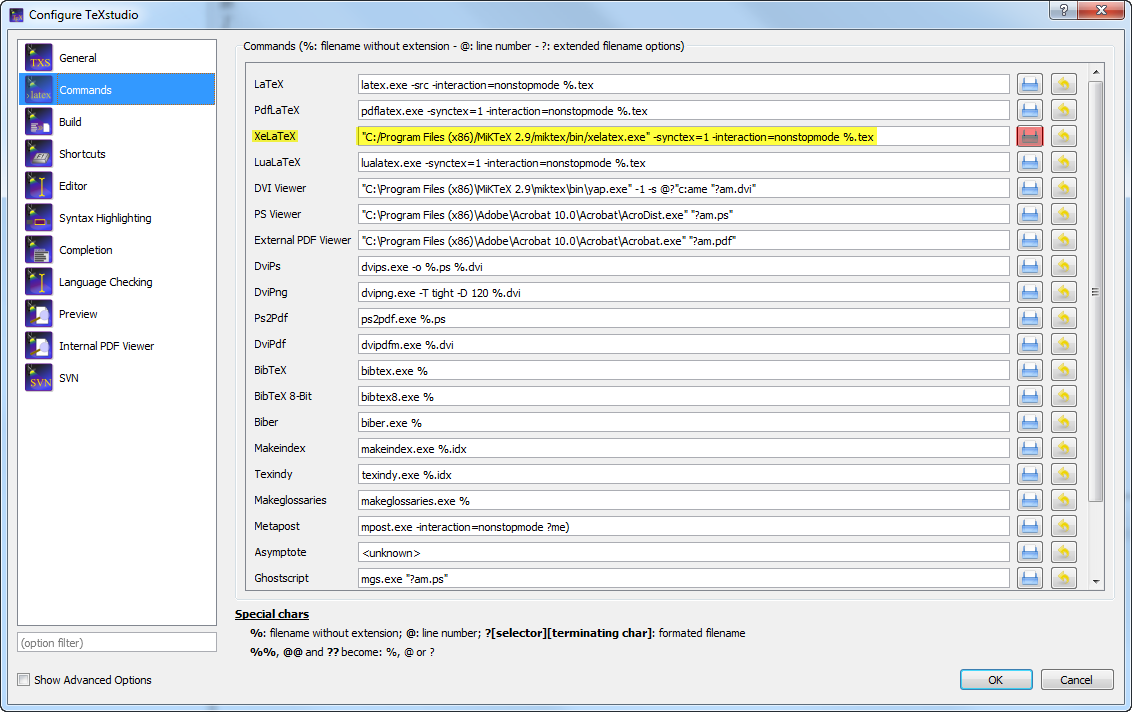
\includegraphics[width=0.5\textwidth]{CompileChange.png}
	\caption{Changing the method of compilation for XeLaTeX in TeXstudio. Also at the bottom of the page.}
	\label{fig:continued_fig}
\end{figure}

This section has filler text. These words serve no meaning except to fill a few lines in the document. This section has filler text. These words serve no meaning except to fill a few lines in the document. This section has filler text. These words serve no meaning except to fill a few lines in the document. This section has filler text. These words serve no meaning except to fill a few lines in the document. This section has filler text. These words serve no meaning except to fill a few lines in the document. This section has filler text. These words serve no meaning except to fill a few lines in the document. This section has filler text. These words serve no meaning except to fill a few lines in the document. This section has filler text. These words serve no meaning except to fill a few lines in the document. This section has filler text. These words serve no meaning except to fill a few lines in the document. This section has filler text. These words serve no meaning except to fill a few lines in the document. This section has filler text. These words serve no meaning except to fill a few lines in the document. This section has filler text. These words serve no meaning except to fill a few lines in the document. This section has filler text. These words serve no meaning except to fill a few lines in the document. This section has filler text. These words serve no meaning except to fill a few lines in the document. This section has filler text. These words serve no meaning except to fill a few lines in the document. This section has filler text. These words serve no meaning except to fill a few lines in the document. This section has filler text. These words serve no meaning except to fill a few lines in the document. This section has filler text. These words serve no meaning except to fill a few lines in the document.

\begin{figure}[ht]
	\ContinuedFloat
	\centering
	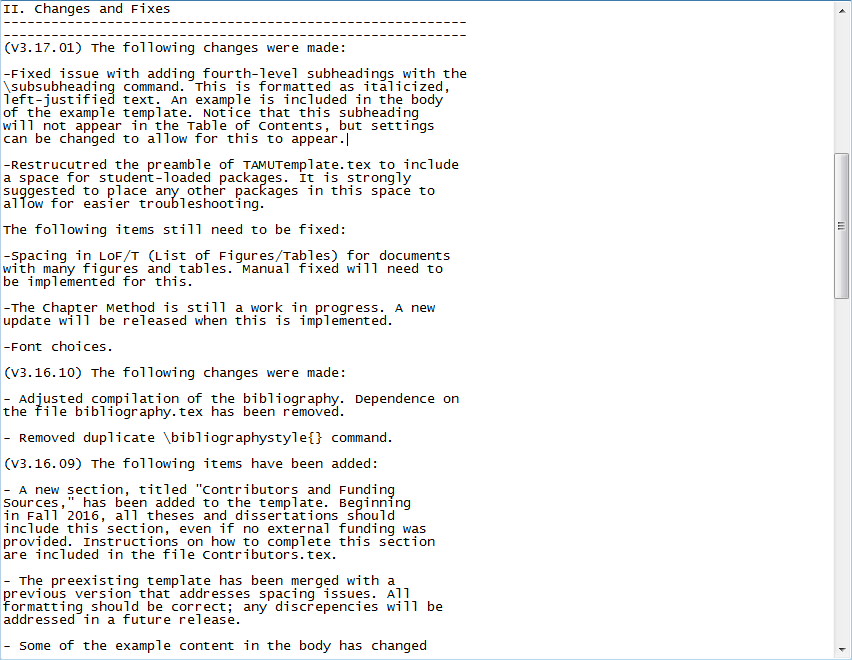
\includegraphics[width = 0.5\textwidth]{Changelog.png}
	\caption[]{Continued.}
\end{figure}

This section has filler text. These words serve no meaning except to fill a few lines in the document. This section has filler text. These words serve no meaning except to fill a few lines in the document. This section has filler text. These words serve no meaning except to fill a few lines in the document. This section has filler text. These words serve no meaning except to fill a few lines in the document. This section has filler text. These words serve no meaning except to fill a few lines in the document. This section has filler text. These words serve no meaning except to fill a few lines in the document.

\section{Challenges}
Section here is to test toc display only.

\section{Further Study}
Section here is to test toc display only.
